\documentclass[10pt]{beamer}


\mode<presentation> 
{
  \usetheme{Diku}
  \beamertemplatenavigationsymbolsempty
  \setbeamercovered{invisible}
%  \setbeamercovered{transparent}
}


\usepackage[danish]{babel}
\usepackage[latin1]{inputenc}
\usepackage{times}
\usepackage[T1]{fontenc}
% \usepackage[english]{babel}
\usepackage{hyperref}
\usepackage{animate}
%\usepackage{multimedia}
\usepackage{francois-preamble}
\usepackage{multirow}
\usepackage{amssymb}

\usepackage{multirow}
%\usepackage{movie15}

\newcommand{\cc}{{c\!\!,}}
\newcommand{\degr}[1]{{{#1}^\circ}}

\title{CNN2}

\author[S. Olsen] % (optional, use only with lots of authors)
{S�ren Olsen}

\institute[DIKU] % (optional, but mostly needed)
{
  Department of Computer Science\\
  University of Copenhagen
}

\date[2015-16 B1] % (optional, should be abbreviation of conference name)
% {Research Presentation, Diku 2006}


% Insert page numbers
\pagenumbering{arabic}
\setbeamertemplate{footline}{\hspace{5pt}\insertpagenumber\vspace{10pt}}


\definecolor{gold}{rgb}{0.95,0.83,0.0}
\definecolor{orange}{rgb}{0.95,0.7,0.0}
% \definecolor{backblue}{rgb}{0.93,0.94,0.99}
\definecolor{backblue}{rgb}{0.95,0.94,0.99}
\setbeamercolor*{background canvas}{bg=backblue} 



\newcommand{\myemph}[1]{{\color{blue}{#1}}}
\newcommand{\intrg}[1]{\int_{{#1}=-\infty}^\infty}
\newcommand{\intRR}{\int_{-\infty}^\infty}

\AtBeginSection[]
{
  \begin{frame}<beamer>{Outline}
    \tableofcontents[currentsection,currentsubsection]
  \end{frame}
}

\begin{document}
\maketitle




%-------------------------------------------------------------------
%   Start slides
%-------------------------------------------------------------------


%-------------------------------------------------------------------
% \begin{frame} 
%   \frametitle{Last week}
%   \begin{itemize}
%   \item Historical frame + Introduction to CNN's  \\[5mm]
%   \item Did you prepare by reading? Did you do the experiment?  \\[5mm]
%   \item Today we will go deeper into convolutions, backpropagation, loss
%     functions, regularization etc. etc. \\[5mm]
%   \end{itemize}
% \end{frame}



%-------------------------------------------------------------------
\begin{frame}
\frametitle{Agenda} 


\begin{itemize}
\item Training, Annotation, Transfer learning
% \item What can a neuron compute ?
% \item FC-net: The Universal approximation Theorem
\item Overfitting
\item Convolutions
\item Optimization: Gradient descent, SGD etc
\item The zoo of network architectures
\item Course evaluation
\end{itemize}
\vspace{4mm}

% I think we wait one/two more week before we go through the
% backpropagation algorithm. % and we start looking in details at dffferenrt nets.

\end{frame}


%-------------------------------------------------------------------
\begin{frame} 
\frametitle{Training}
To train the net (or estimate the value of the many parameters) these
may be randomly initialized. Then an image is processed and the
resulting error (difference between output and annotation) is
recorded. Now a version of {\color{blue}{the backpropagation algorithm}}
is used to change all parameter values.  \\[4mm]

This is repeated many times for a huge amount of annotated images
spanning all the possible ways these may look. \\[4mm]

Quite advanced numerical algorithms are used for training. Training
may take from hours to weeks on a GPU.  Without, it may (in many
cases) not be realistic. Training may be complicated and involve a lot
of tricks. If not done correctly training often fails.
\end{frame}



%-------------------------------------------------------------------
\begin{frame} 
\frametitle{Annotated data}
A major obstacle in CNN usage is to establish large enough annotated
data. Acquirering the images itself may be difficult.  However human
annotation (e.g. marking bounding boxes and writing class label) may
take more time than the actual training. \\[4mm]


Say that you can annotate an image with on average 10 items 
within one minute.  Say that you for a 2M parameter net need 10 times
as many training data.  Then you have to work 2M
minutes or 556 hours or about 14 weeks (40 efficient hours a
week). 
\end{frame}



%-------------------------------------------------------------------
\begin{frame} 
  \frametitle{Annotation problems and solutions}
One solution is to use a {\color{blue}{Mechanical Turk}}, i.e. to pay
other people to do the annotations. This may quickly give many
annotations. \\[3mm]
  
One problem in annotation is that this may be incorrect: Wrong label,
badly placed bounding box or missing identification. Often people
annotate differently.  This will severely hurt the learning
process. Correcting false annotations is a pain. \\[3mm]

In some cases, use of (photo-realistic) synthetic images may solve
the problem of getting enough annotated date. This approach has shown
possible within semantic segmentation of street scenes, and
classification of plants.
  
\end{frame}



%-------------------------------------------------------------------
\begin{frame}
  \begin{center}
    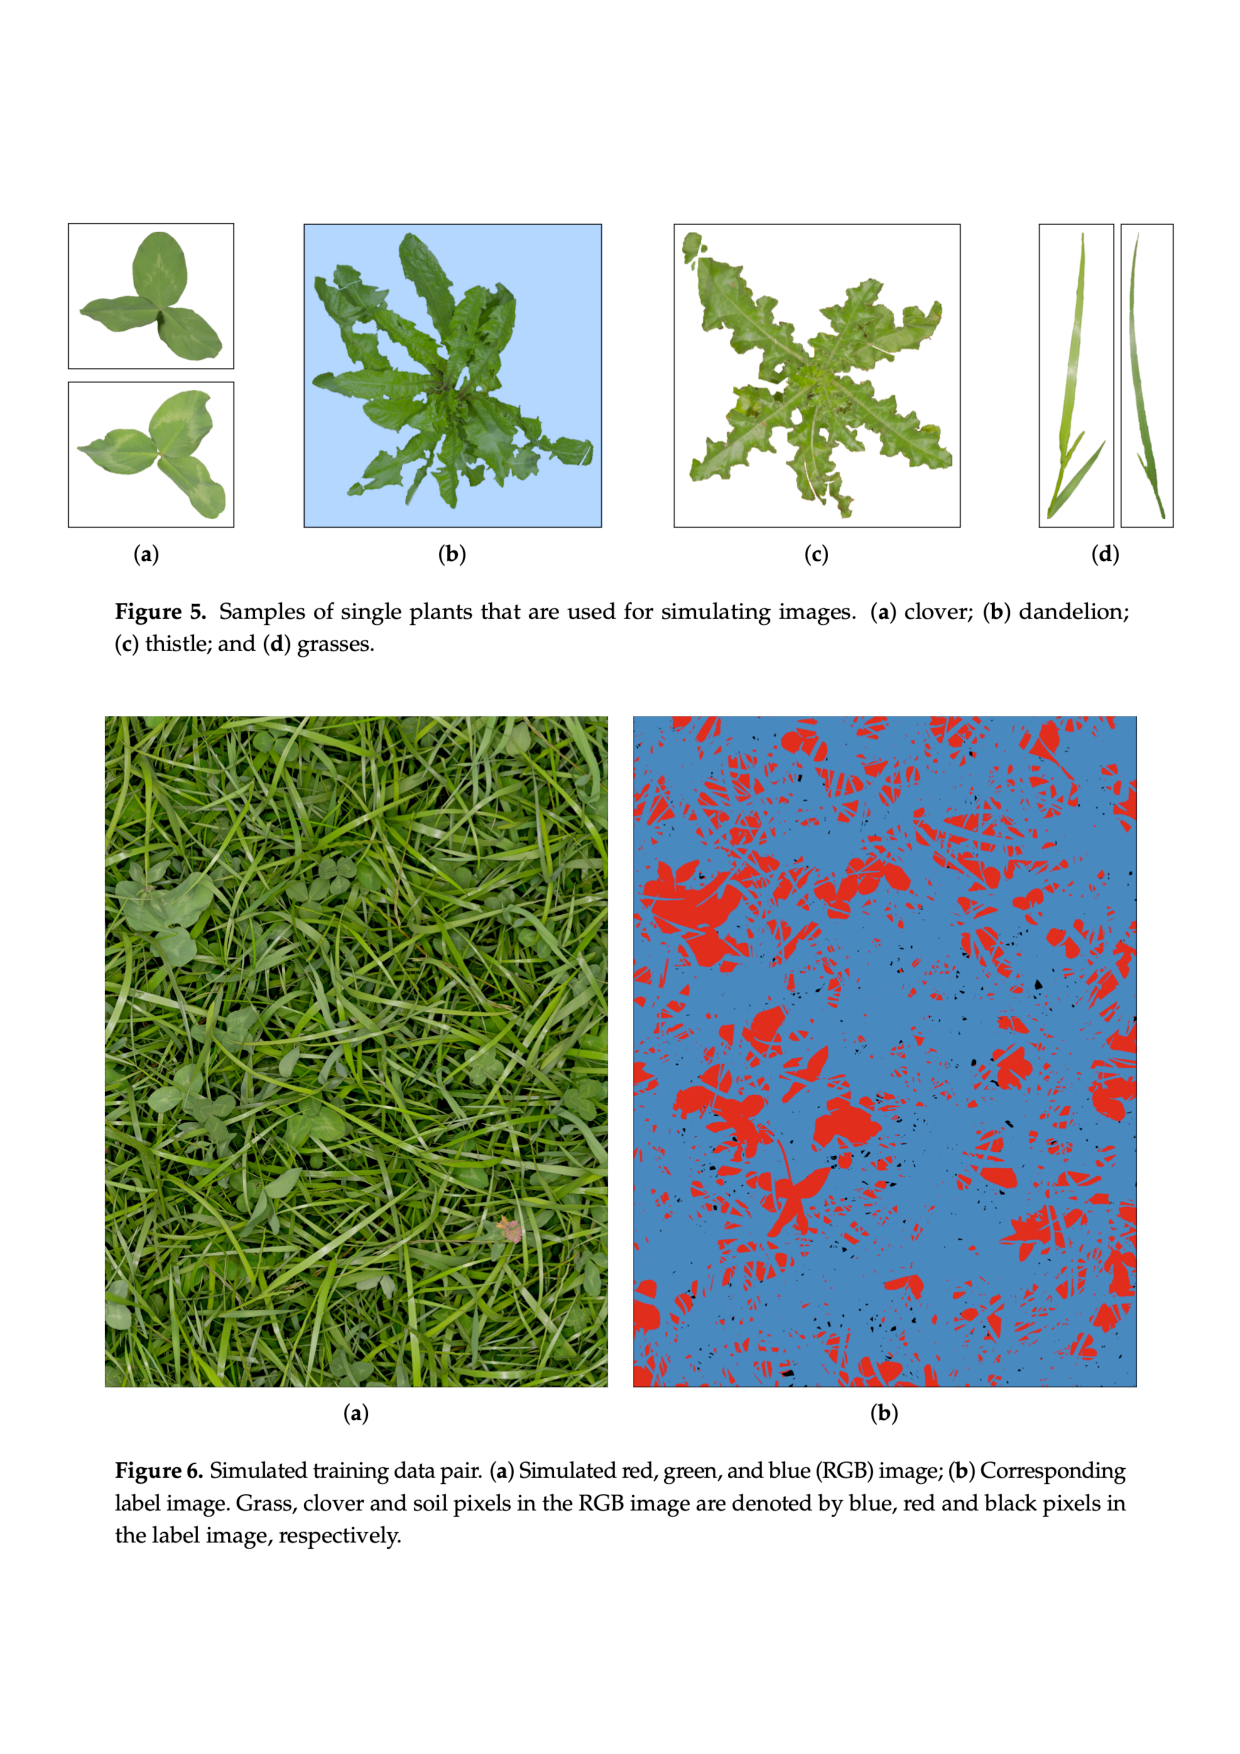
\includegraphics[width=70mm]{Images/SyntImage.pdf}
    \end{center}
\end{frame}



%-------------------------------------------------------------------
\begin{frame}
  \begin{center}
    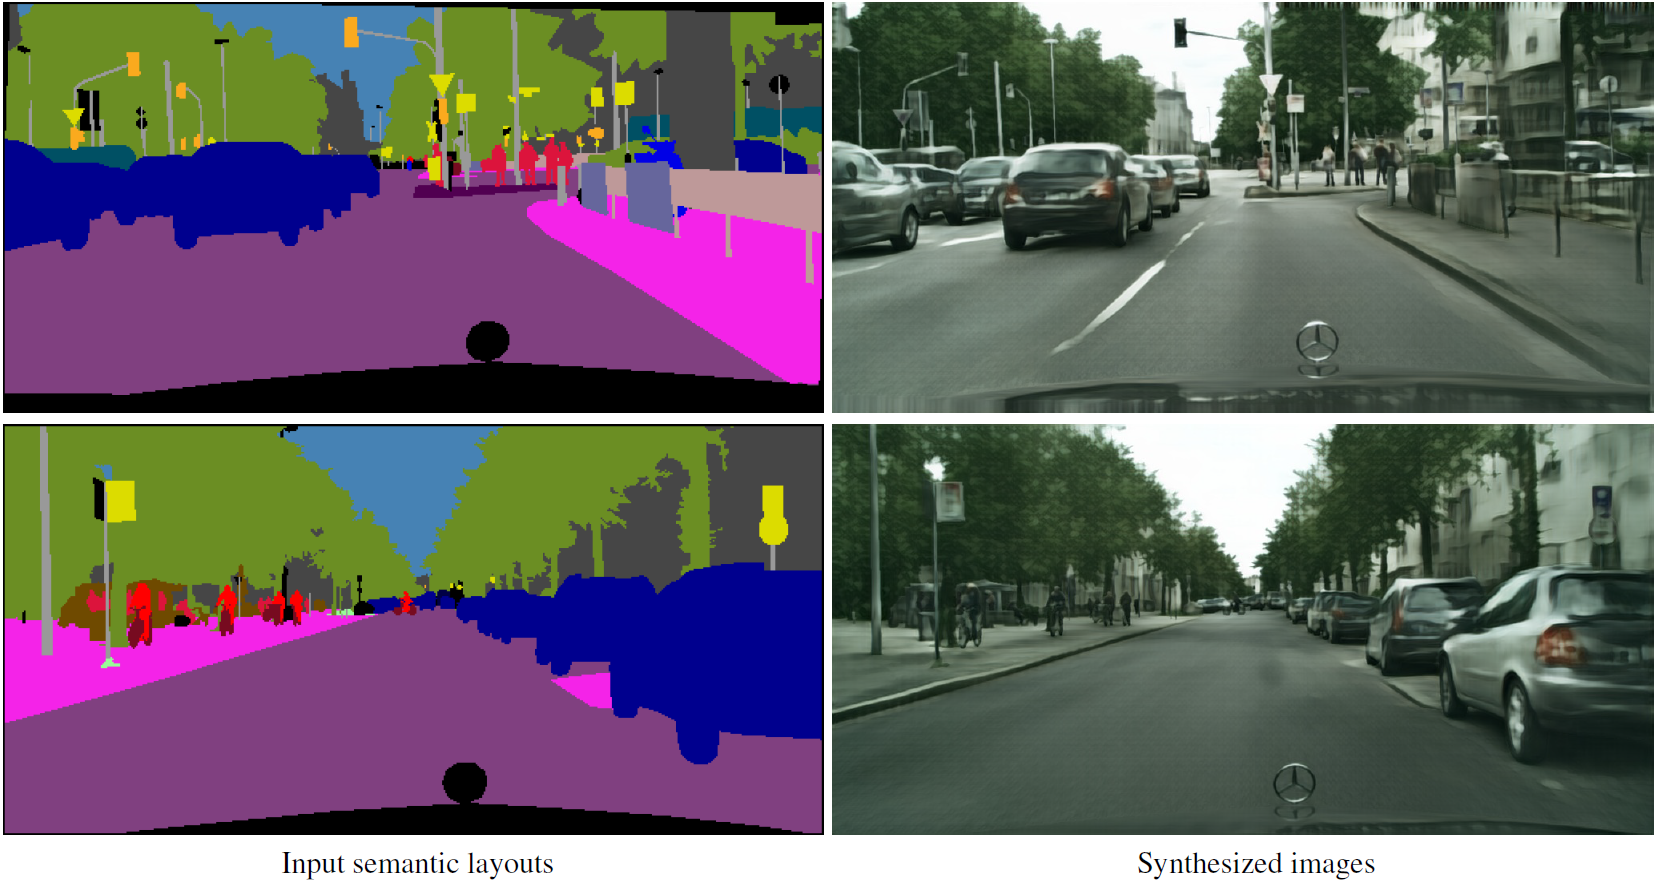
\includegraphics[width=100mm]{Images/SynStreetImage.png}
    \end{center}
\end{frame}



%-------------------------------------------------------------------
\begin{frame} 
  \frametitle{Transfer learning}

  A number of networks (say for recognition of different classes of
  objects) may share the backbone network. In this cases, if a good
  net exist, the trained parameters may be borrowed. \\[5mm]

  Many of the more famous nets, and their parameters, are publicly
  available. Then fine-tuning on a new (and much smaller) data set
  may result in fast and easy learning.  \\[5mm]

  In some cases only the FC-layers may need redesign- and training.
  This limits the need for huge amounts of annotated data.
\end{frame}




%-------------------------------------------------------------------
% \begin{frame} 
%  \frametitle{}
%  \begin{center}
%     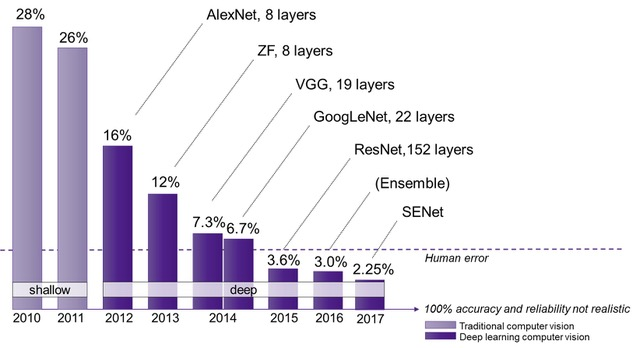
\includegraphics[width=100mm]{Images/ImageNetResults.jpeg}   
%   \end{center}
% \end{frame}



%-------------------------------------------------------------------
% \begin{frame} 
%   \frametitle{Neuron = Classifier}
% An artificial neuron (excl. non-linear operation) computes a linear
% combination of the input.  If $N$ input values this is the (scaled)
% perpendicular distance of the $N$-dimensional input point to the
% straight line defined by the weights $w$. \\[4mm]
%
% Adding nonliniarity e.g. a arctan, the neuron classifies (by positive/negative
% values) the point to be one side of the line. \\[4mm]
%
% Stacking arrays of neurons (classifiers) allows approximate segmention
% of any sub-region in $\mathbb{R}^n$. If region is not smooth, many
% (infinite) neurons are needed.
%
% \end{frame}



%-------------------------------------------------------------------
% \begin{frame}
%  \begin{center}
%    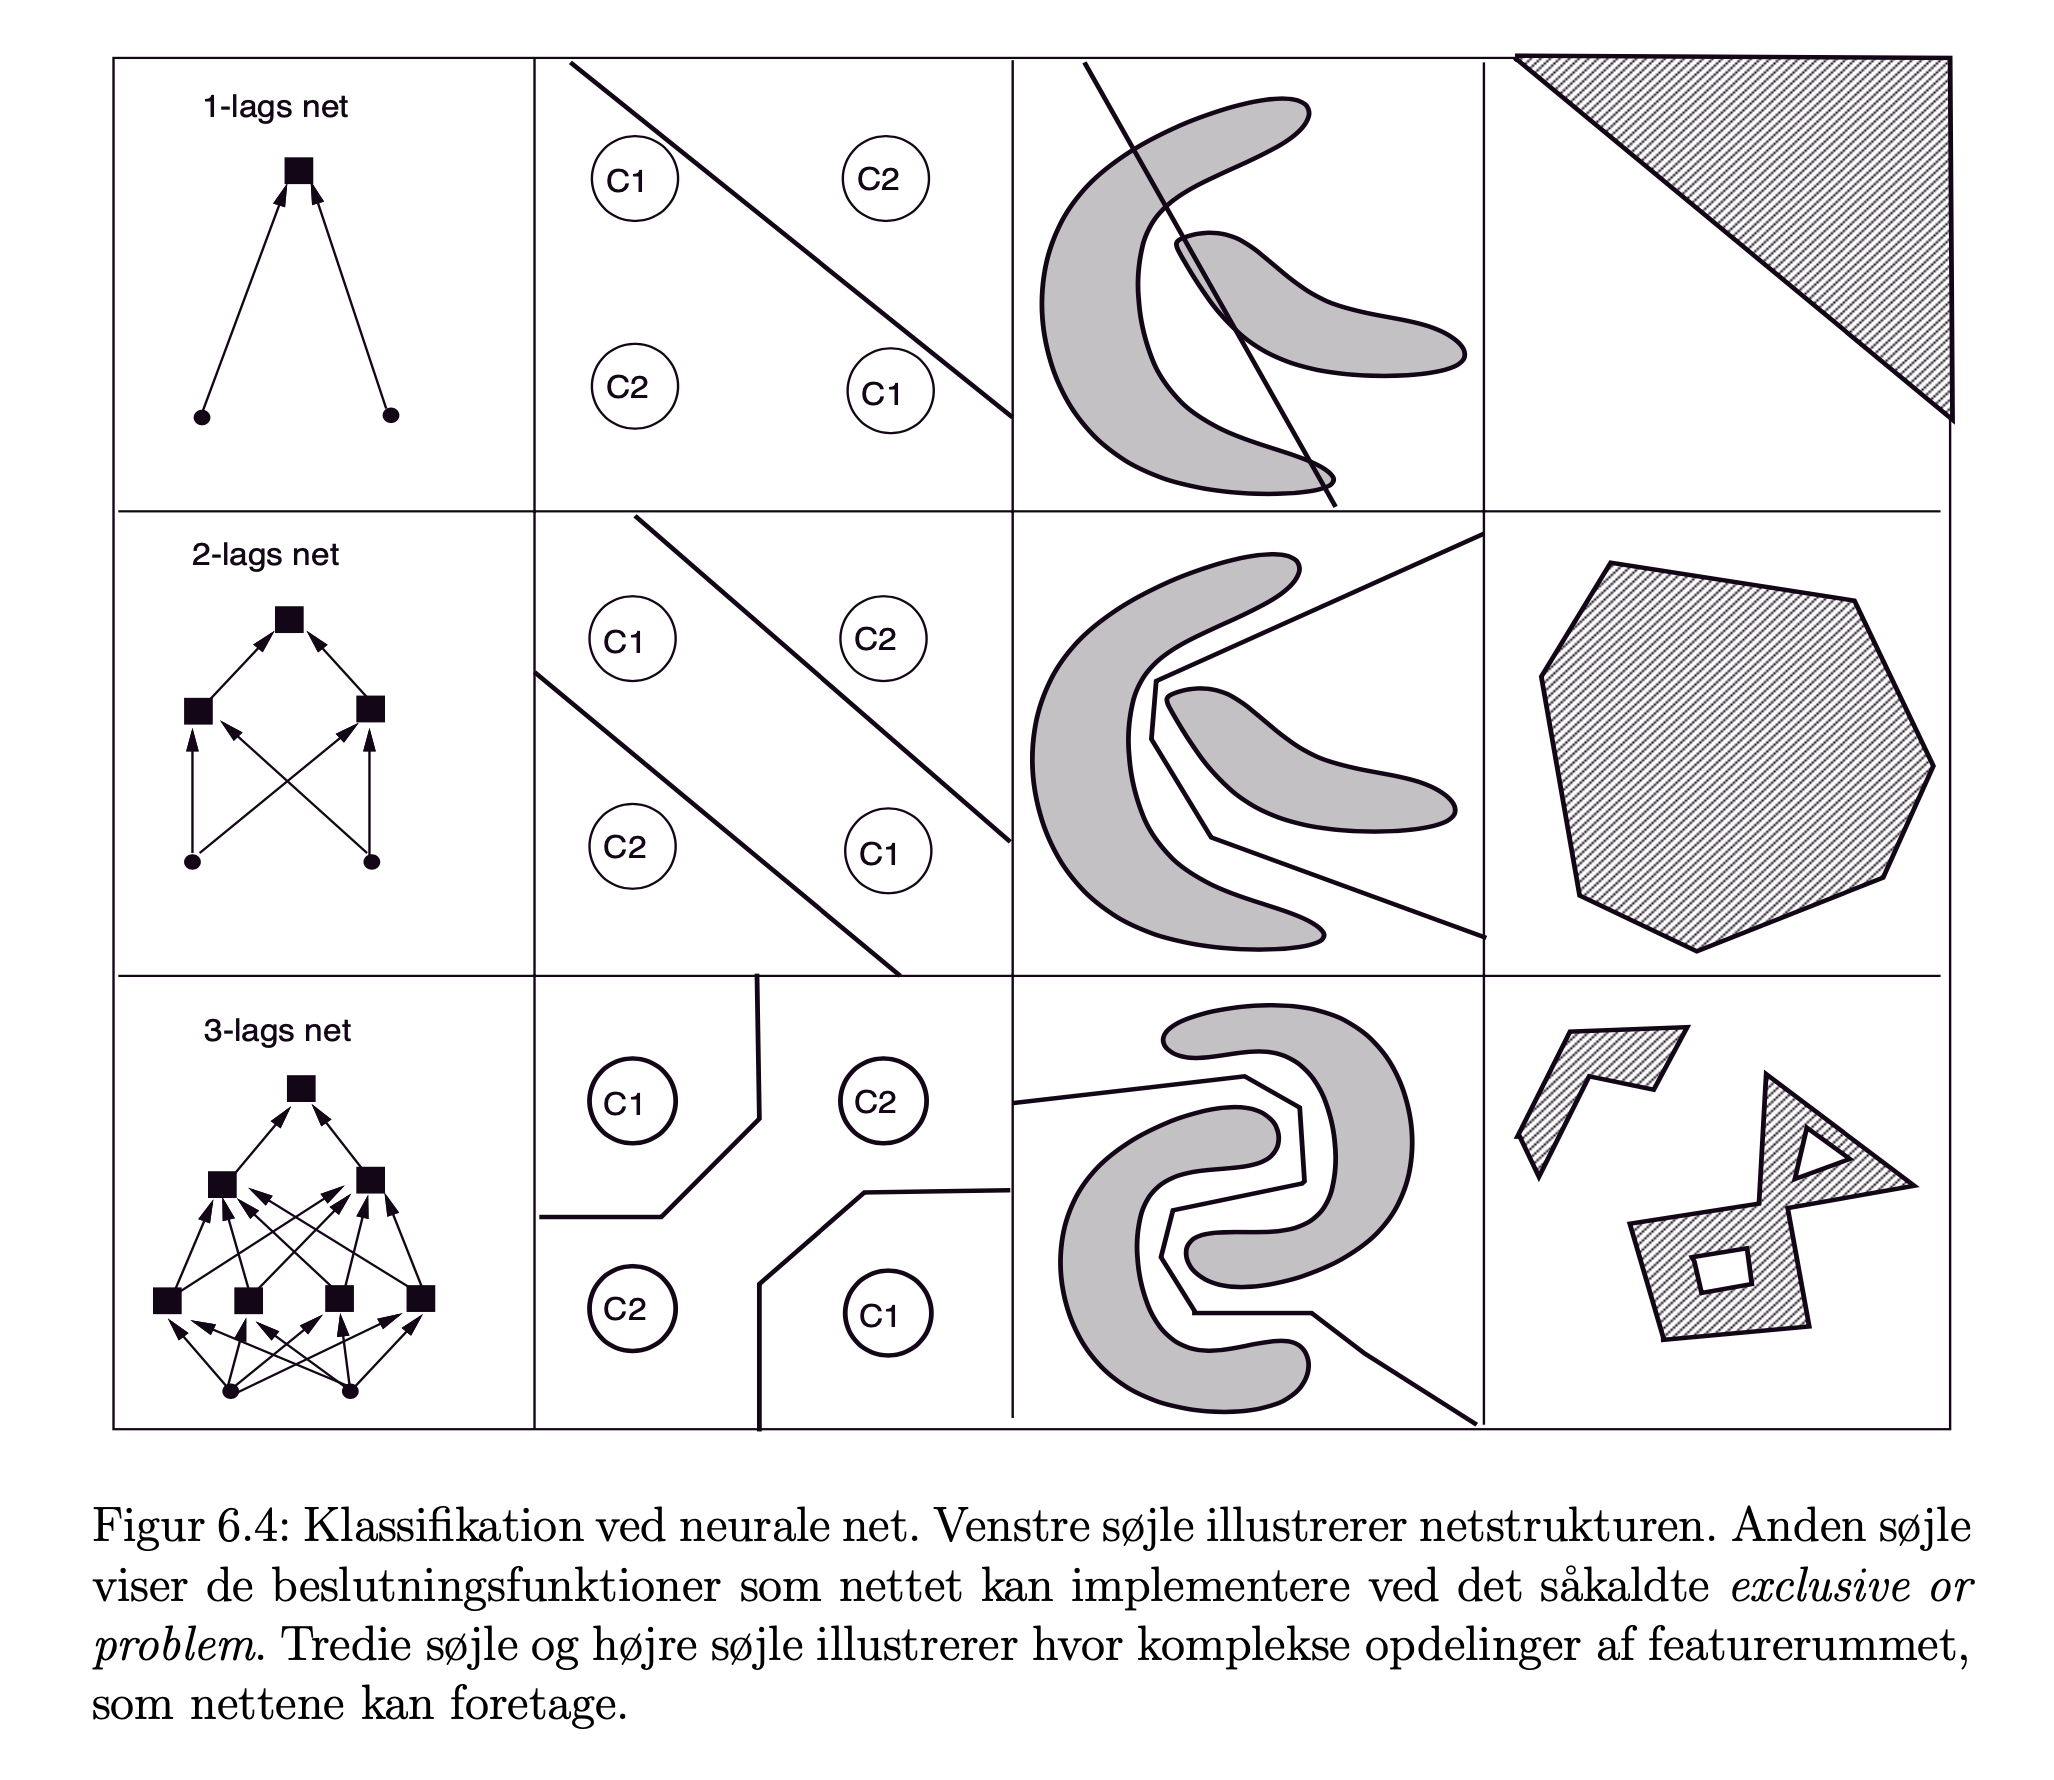
\includegraphics[width=95mm]{Images/NNclass1.png}
%  \end{center}
% \end{frame}



%-------------------------------------------------------------------
% \begin{frame} 
%   \frametitle{Neuron = Approximator}
% Ignoring any non-linear transformation, the neuron approximates a
% linear function in $N$ input values. Thus, any more complicated
% function may not be modelled. \\[3mm]
%
% Combining the output of many neurons, a piecewise linear function may
% be approximated. \\[3mm]
%
% If we want to do better, what do we then need ? More neurons or more
% layers ?  \\[3mm]
%
% Example: Given historical climate data a NN may regress future climate
% (only if training data is representative). \\[3mm]
%
% Example: Given a feature pyramid hierarchi and a anchor position for
% an object detection, regress the 4 bounding box parameters. 
% \end{frame}


%-------------------------------------------------------------------
% \begin{frame} 
%   \frametitle{The Universal approximation theorem}
%   The theorem (See {\em Honik:Approximation Capabilities of Multilayer
%     feedforward Networks}, Neural Networks 4(2), pp. 251-257, 1991) 
% states that under mild assumptions on the activation function,
% {\color{red}{a two layer feed-forward network with sufficiently many
%     neurons may appriximate any continuous function}} (on a compact
% subset of $\mathbb{R}^n$).\\[3mm]
%
% In practice {\color{red}{sufficiently many}} (but not infinitly many) may turn
% out to be pretty large. Also, no guidance on how to train such a net
% is provided. \\[3mm]
%
% The activation function needs to be non-linear, and different from any
% polynomial. \\[3mm]
%
% Later results have shown that a net with sufficient many layers with
% only $n+1$ neurons also may approximate any continuous function of
% $n$-dimensional input variables.
% \end{frame}



%-------------------------------------------------------------------
% \begin{frame} 
%   \frametitle{and more - for the mathmaticians}
% In 2017 Lu et al. (See Wikipedia)  proved a universal approximation
% theorem for width-bounded deep neural networks. In particular, they
% showed that width-$n+4$ networks with ReLU activation functions can
% approximate any Lebesgue integrable function on $n$-dimensional input
% space with respect to $L^1$  distance if the network depth is allowed
% to grow. They also showed the limited expressive power if the width is
% less than or equal to n. All Lebesgue integrable functions except for
% a zero measure set cannot be approximated by width-$n$ ReLU
% networks. \\[4mm] 
%
% A later result (See Wikipedia) showed that ReLU networks with width
% $n+1$ is sufficient to approximate any continuous function of
% $n$-dimensional input variables.
%
% \end{frame}



%-------------------------------------------------------------------
% \begin{frame} 
%   \frametitle{Neuron = Correlator = feature detector}
% The cross-correlation between two real-valued vectors $x$ and $w$ is
% defined by their dot-product, i.e. just what a neuron does. \\[4mm]
%% {\color{red}{draw}}.
%
% The cross-correlation value is (numerical) large when the
% vectors/functions fit (are equal) and is zero when the vectors are
% orthogonal. Thus, the filter $w$ acts as a prototype/template, and the
% neuron response is the degree of fit. \\[4mm]
%
% If the vectors are normalized w.r.t. mean and standard deviation, the
% cross-correlation $\in [-1:1]$, with $-1$ as a sign-reversed perfect
% fit. 
% \end{frame}



%-------------------------------------------------------------------
% \begin{frame} 
%   \frametitle{Correlations}
% The correlation between two 1D real-valued continuous functions $f(x)$
% and $g(x)$ is a new real-valued continuous function $h(x)$ defined by:
%
% \begin{displaymath}
%   h(x) \;=\; \int_{t= -\infty}^{\infty} f(x+t) g(t) dt
% \end{displaymath}
%
% The definition directly translated to the discrete version. Note the
% symmetry between $f$ and $g$.  If we think of $g$ as a filter with
% support $[0:N]$, we have:
%
% \begin{displaymath}
%   h[x] \;=\; \sum_{t=0}^{N} f[x+t] g[t]
% \end{displaymath}
%
% Recognize that correlations are just a linear combination of the input
% values $f[x]$ given by the weights $g[x]$.
% \end{frame}


%-------------------------------------------------------------------
% \begin{frame}
% Cross correlation of two discrete functions $f[x]$ and $g[x]$ is
% defined by:
%
% \begin{displaymath}
%   r[x] \;=\; \sum_i f[x+i] g^{\star}[i]
% \end{displaymath}
% where $g^{\star}$ is the complex conjugate of $g$. For real valued
% functions its identical to $g$. {\color{blue}{Normalized cross correlation}}
% is defined by:
%
% \begin{displaymath}
%   r[x] \;=\; \sum_i \frac{(f[x+i] - \mu_f)  (g^{\star}[i] -
%     \mu_g)}{\sigma_f \; \sigma_g}
% \end{displaymath}
% where $\mu$ is the average and $\sigma$ is the standard
% deviation. \\[4mm]
%
% The expression is easily extended to 2D, in which case $r[x][y]$ will
% be an image of normalized cross correlation values.
% \end{frame}


%-------------------------------------------------------------------
% \begin{frame}
%     \begin{center}
%     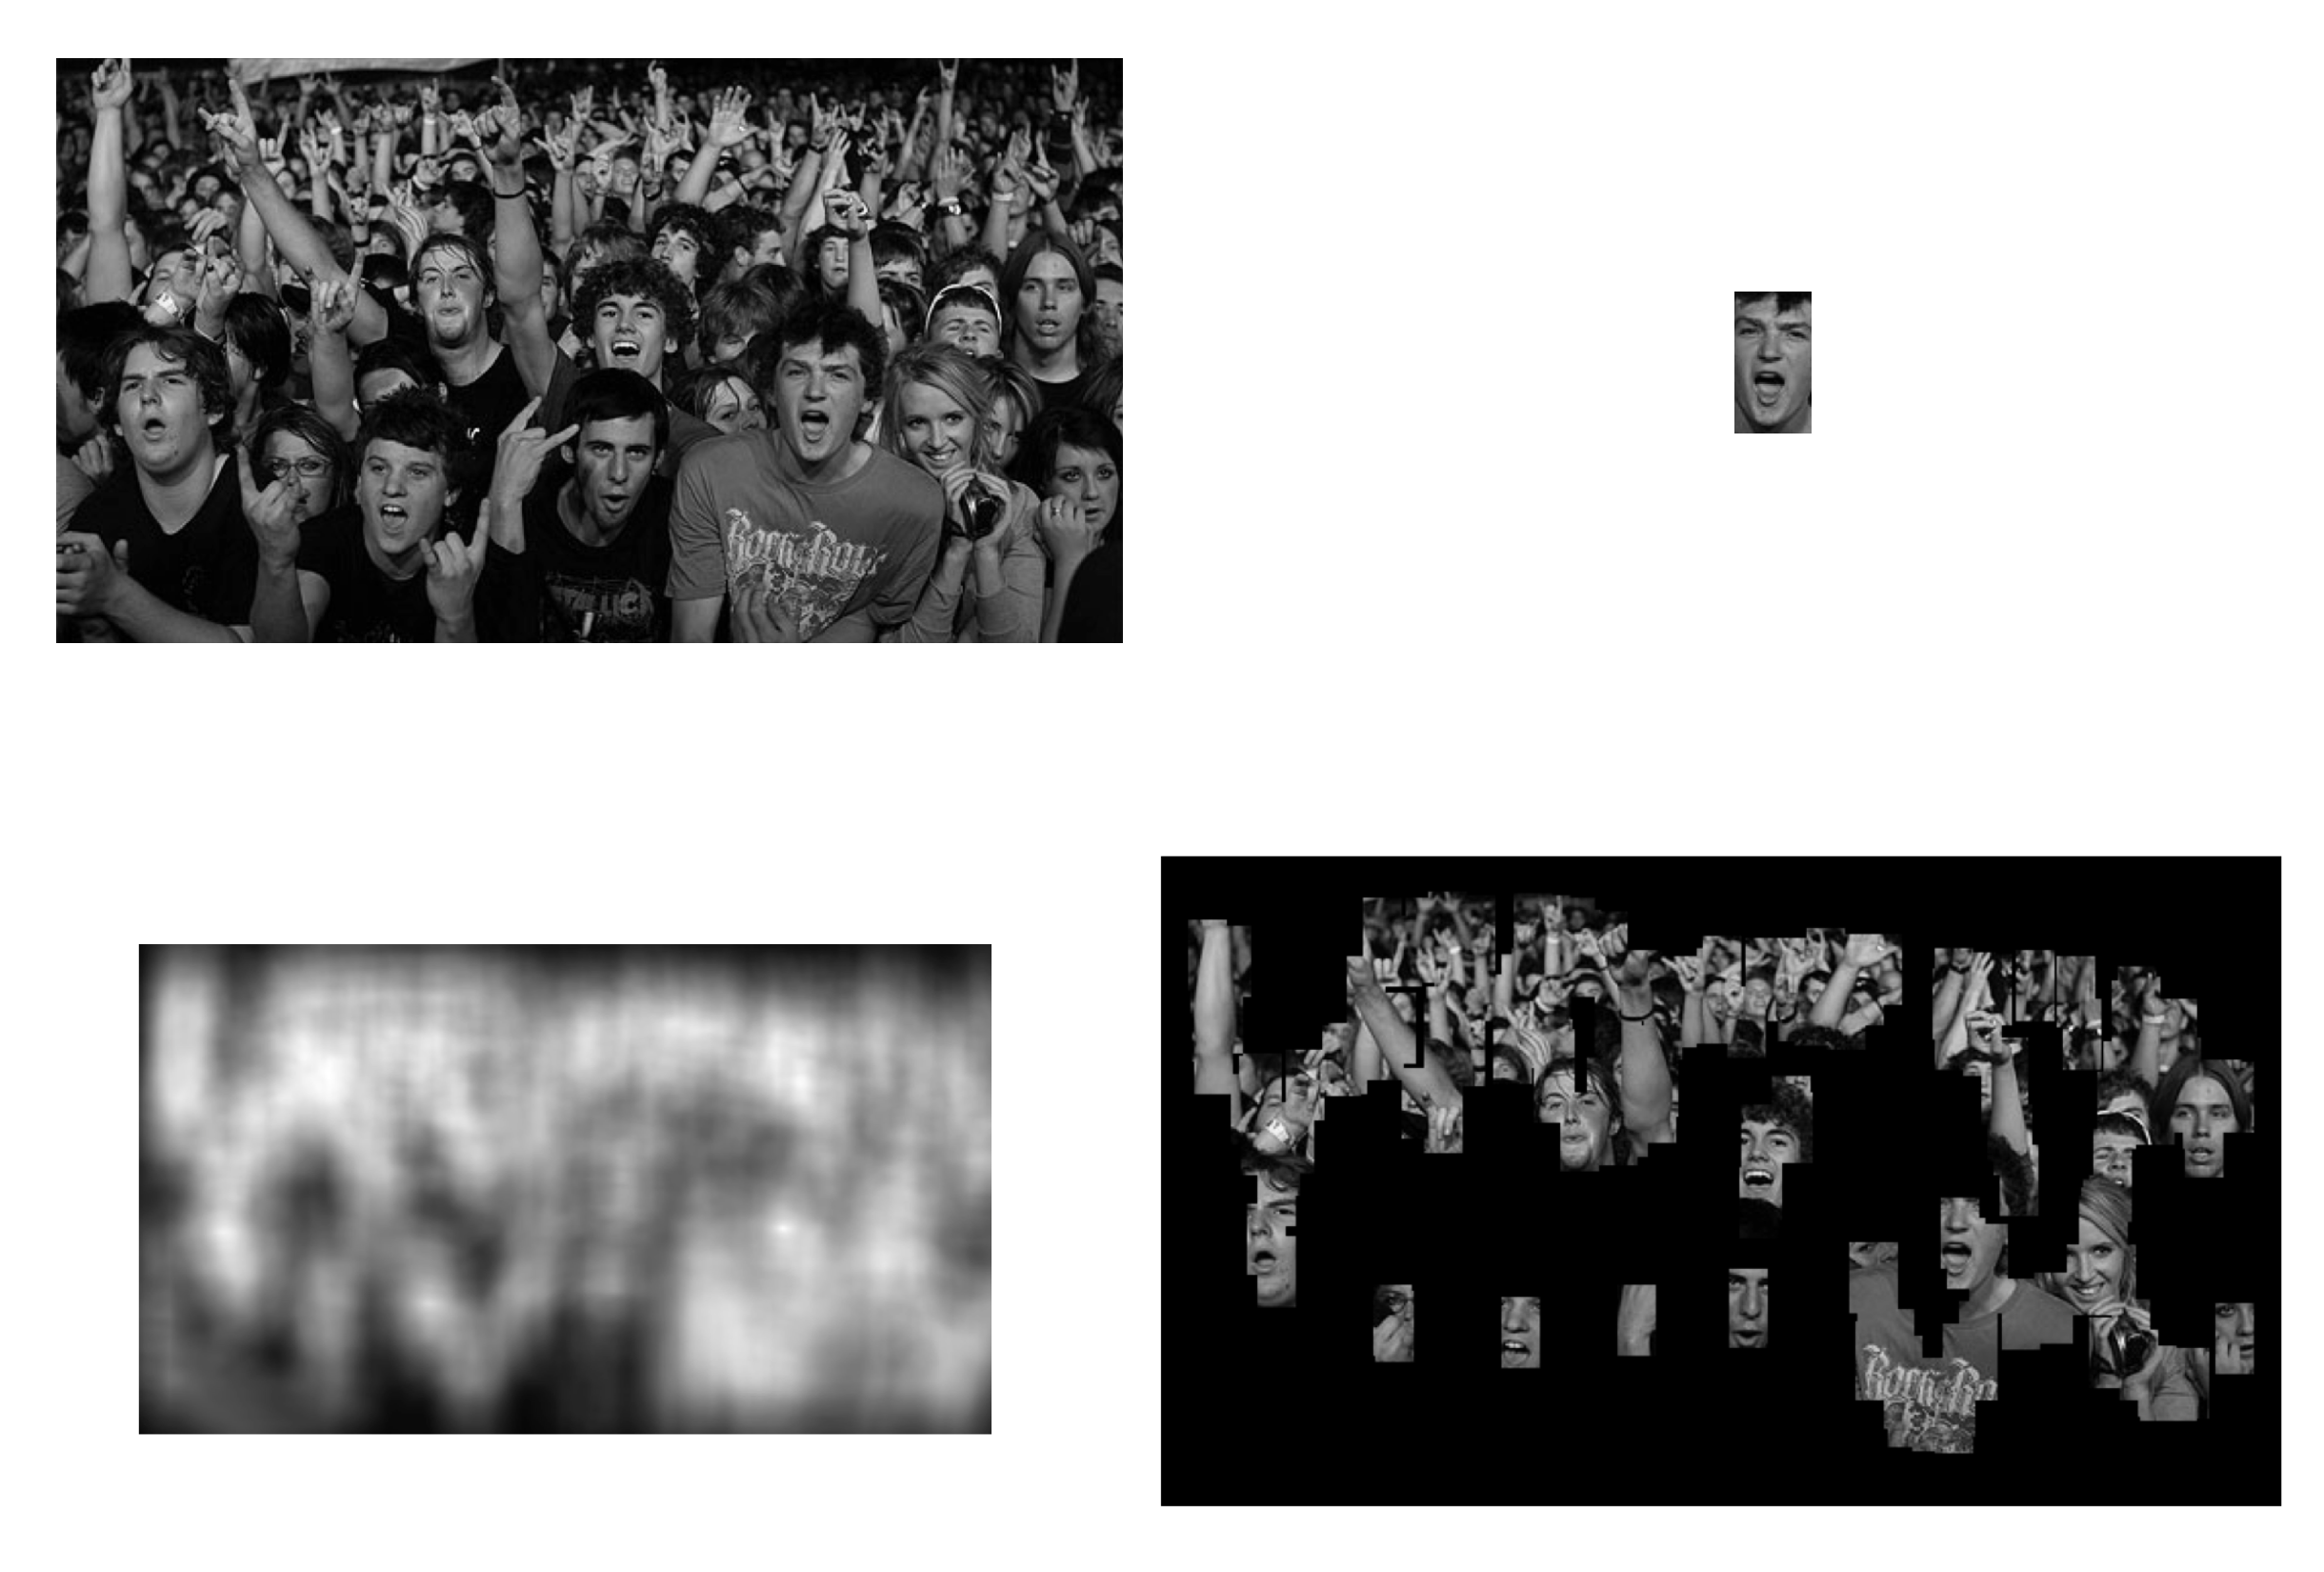
\includegraphics[width=100mm]{Images/CrosscorrEX1.png}
%   \end{center}
%
%   An example of normalized cross correlation. The lower left image
%   could resemble the result of an CNN-filter.
% \end{frame}


%-------------------------------------------------------------------
% \begin{frame} 
% Correlations/convolutions are used in "`matched filtering"' where we
% search for a maximum response to a fit to the filter.
%
% \begin{center}
%   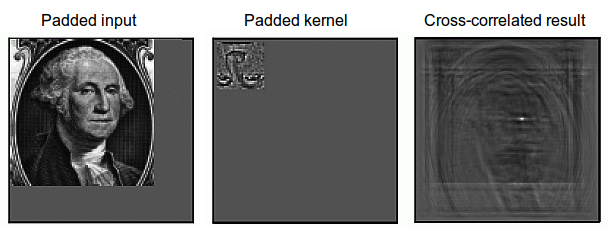
\includegraphics[width=90mm]{Images/crosscorrelation_Example.png}   
% \end{center}
%
% Conceptually, this is just what we need. \\[2mm]
%
% How many neurons do we need to detect specific objects and what
% happens if we choose too few or too many ?
% \end{frame}


%-------------------------------------------------------------------
% \begin{frame}
%   In simple CNN's neureons often play the role as feature
%   detctors. However, their ability (depending on the activation
%   function) to act as approximators or discriminators are important to
%   keep in mind. \\[8mm]
%
% {\color{blue}{\large How many neurons do we need. What
%       happens if we choose too few or too many?}}
% \end{frame}


%-------------------------------------------------------------------
\begin{frame} 
  \frametitle{Fitting/overfitting and model selection}
  Assume that we want to fit a polynomium (in 1 variable $x$) to $n$
  data points.  What order $d$ of the polynomial should we use, i.e.
  how many parameters
% $ \left ( \begin{array}{c} 1+d \\ d \\ \end{array} \right )$ are
needed.\\[5mm]

\begin{itemize}
\item If too few, we cannot model well and the fit will be bad \\[3mm]
\item Remember that all data er noisy \\[3mm]
\item If too high order, overfitting takes place ({\color{red}{draw}}). \\[3mm]
\item How do we know if overfitting occurs ?
\end{itemize}
  
\end{frame}


%-------------------------------------------------------------------
\begin{frame}
 \frametitle{Overfitting - Exampel}

 \begin{center}
   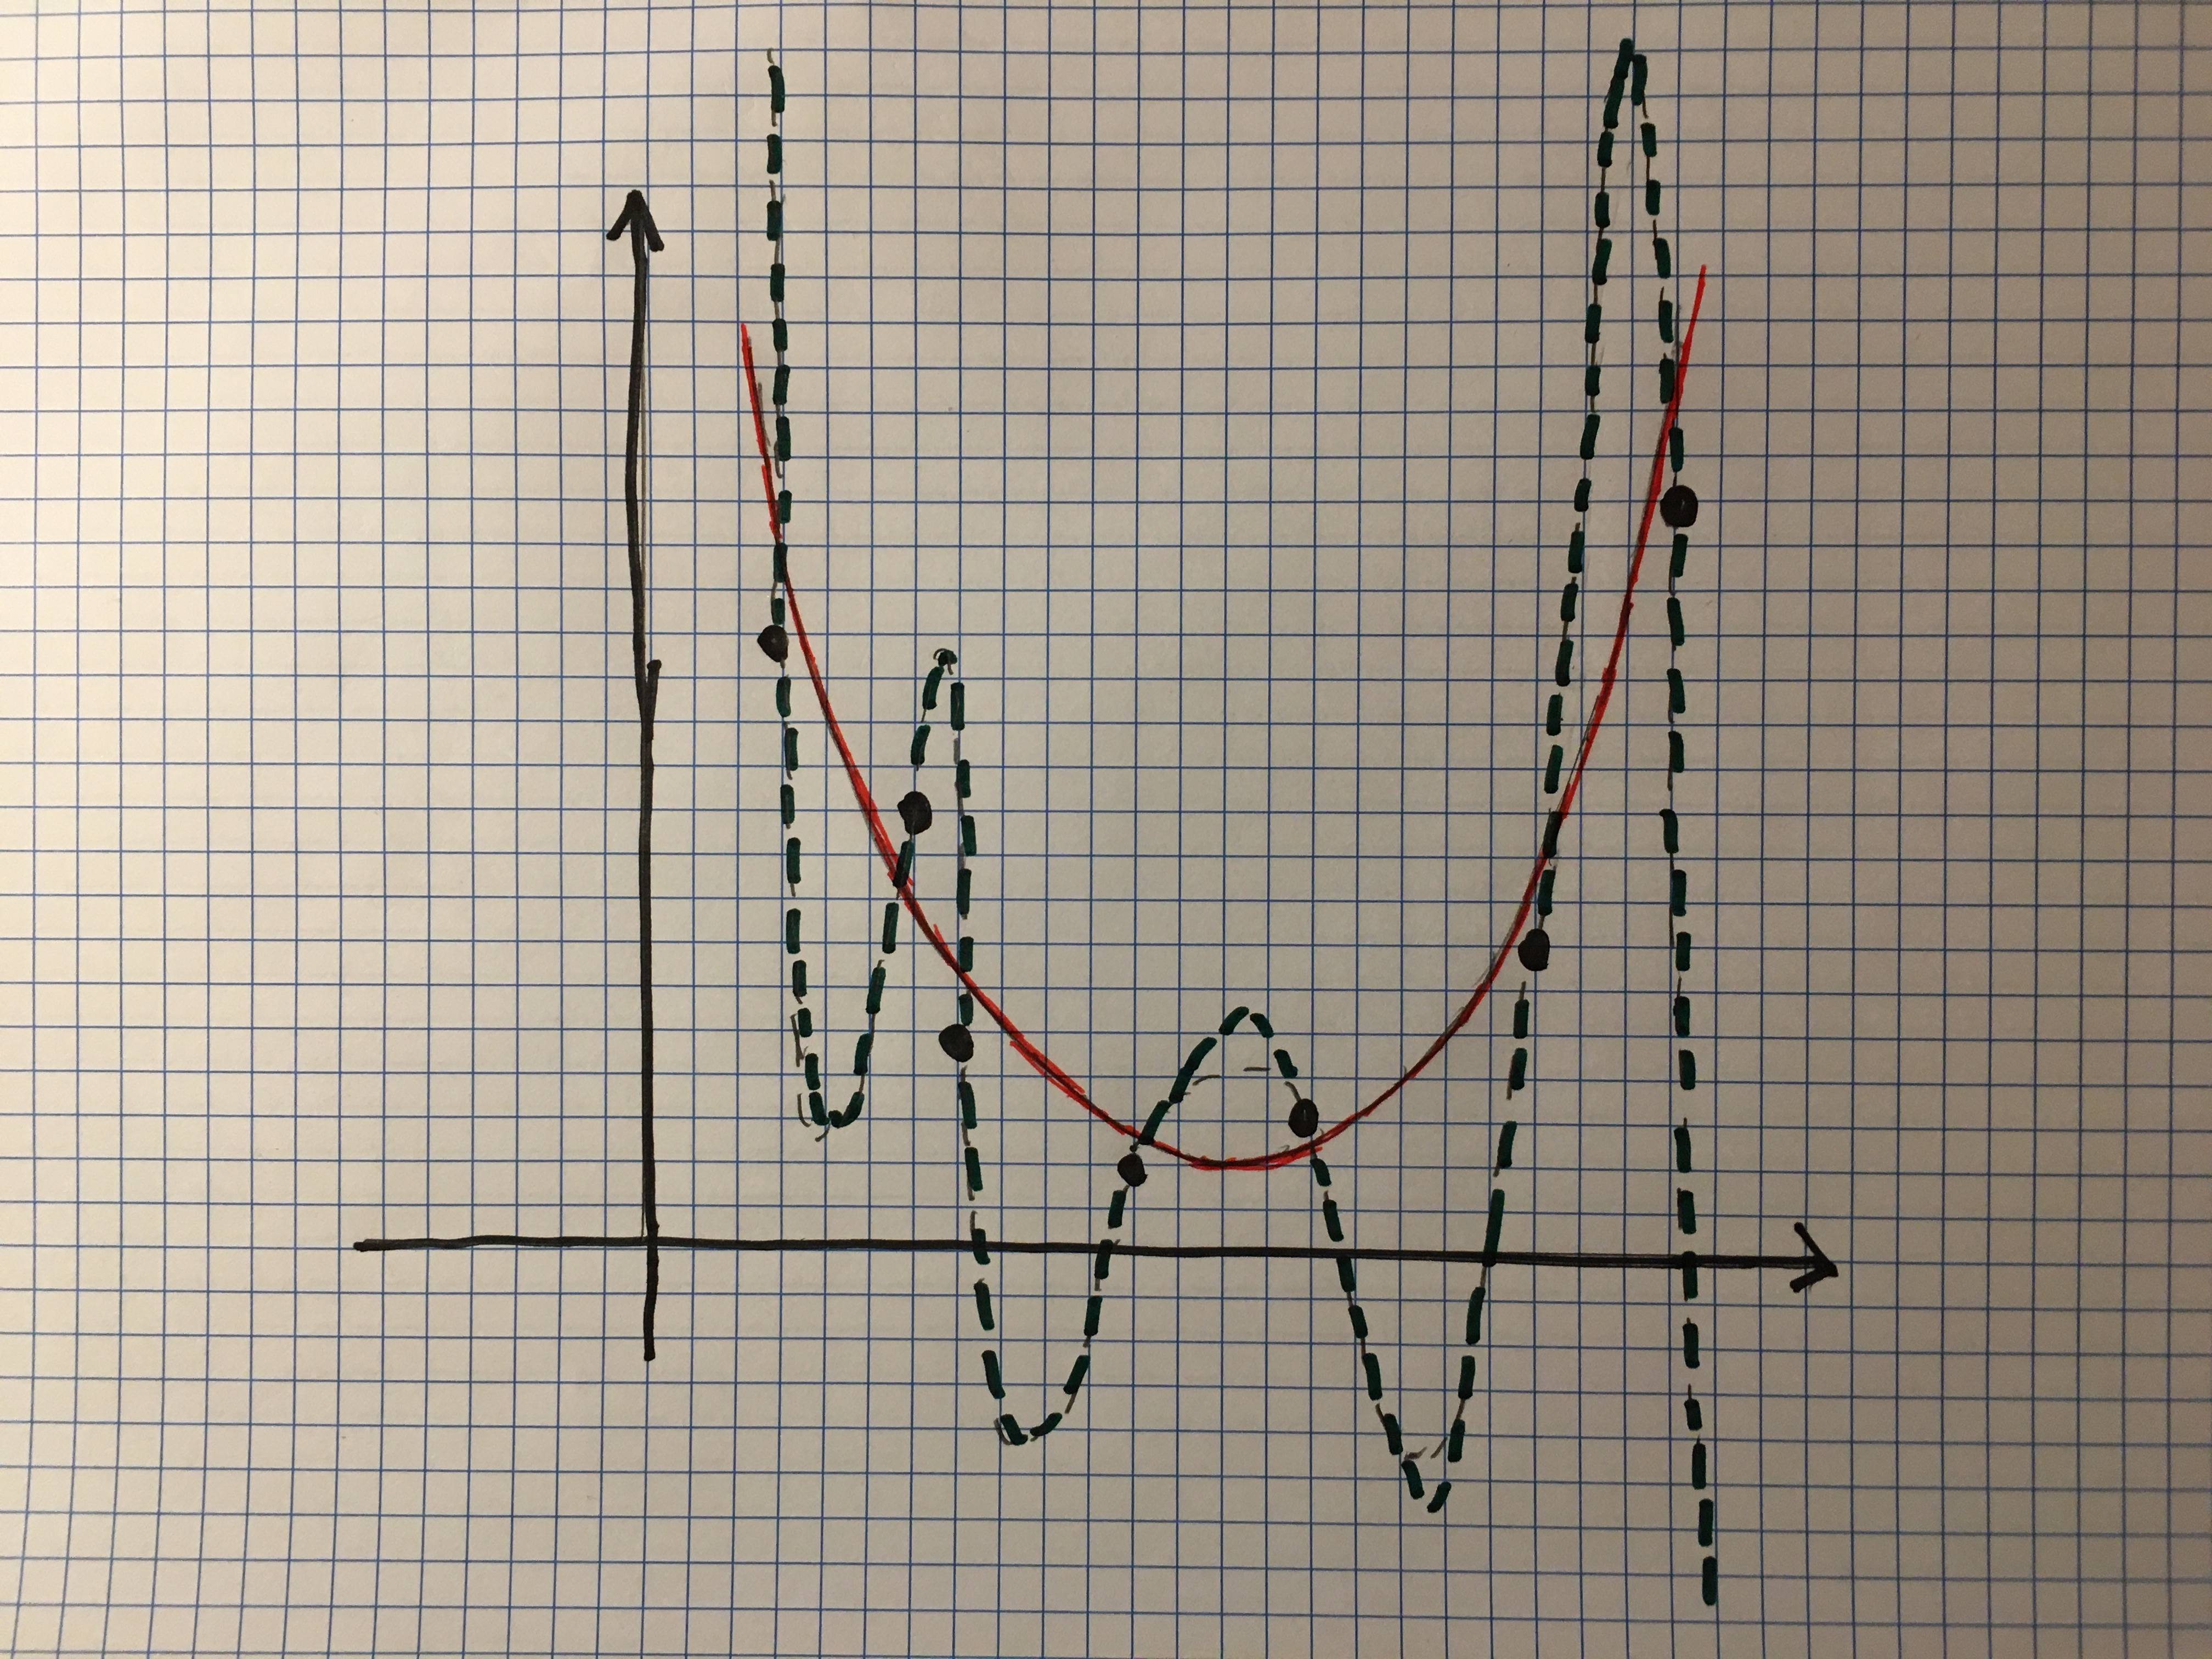
\includegraphics[width=100mm]{Images/IMG_3300.JPG}
 \end{center}

  
\end{frame}


%-------------------------------------------------------------------
\begin{frame} 
 \frametitle{Overfitting}
Neural nets (of any kind) models by applying an exorbitant high number
of parameters.  Thus overfitting is likely to occur. \\[5mm]

A large number of techniques and tricks are applied to avoid/reduce
overfitting.
\begin{itemize}
\item Node pruning
\item Weight sharing (CNN)
\item Dropout
\item Batch- (and other types of) normalization
\item Early stopping
\item Data augmentation
\item Adversarial training
\item etc
\end{itemize}
\end{frame}



%-------------------------------------------------------------------
%  \begin{frame} 
%   \frametitle{Regularization}
% A classical approach to avoid overfitting is to add a regularizing
% term to the objective function penalizing the number of parameters or
% the departure from smoothness (often measured by a sum of gradient
% magnitudes). \\[6mm]
%
% Such approaches are only partially applicable for CNN's, and often
% computationally costly. \\[6mm]
%
% We will later dive deeper into the different regularization methods.
% \end{frame}


%-------------------------------------------------------------------
% \begin{frame} 
%   \frametitle{Convolutions}
% Convolutions are very similar to correlations. A 2D discrete
% convolution is defined by:
%
% \begin{displaymath}
%   h[x][y] \;=\; \sum_{i=0}^{N} \sum_{j=0}^{N} f[x-i][y-j] g[i][j]
% \end{displaymath}
% Thus, the difference is a mirroring of $f$. \\[3mm]
%
% For continuous/discrete functions there exist a number of mathematical
% results (often involving {\color{red}{The Fourier transform}}).  Take
% the course {\color{blue}{Signal and Image Processing}} for more
% information. \\[3mm]
%
% In {\color{red}{Convolutional}} Neural nets (CNNs), we really apply a
% correlation and not a convolution.  \\[3mm]
%
%In all image analysis (classical or modern) convolutions are a core tool.
% \end{frame}


%-------------------------------------------------------------------
% \begin{frame}
% Convolutions are the most applied operation in image processing, no
% matter if we want to do smoothing, contrast enhancement, edge
% detection, gradient computation etc etc.  \\[3mm]
%
% There exist a rich mathematical foundation for convolutions, e.g.:
% \begin{itemize}
% \item $f \star g \;=\; g \star f$
% \item $f \star (g \star h) \;=\; (f \star g) \star h$
% \item $f \star (g + h) \;=\; f \star g + f \star h$
% \item $ D (f \star g) \;=\; Df \star g \;=\; f \star Dg$
% \item $\mathcal{F} (f \star g) \;=\; \mathcal{F}f \cdot \mathcal{F}g$
% \end{itemize}
% \medskip
%
% where $D$ is a differential operator and $\mathcal{F}$ is the
%{\color{blue}{Fourier transform}}.  And there are more, but ...
% \end{frame}



%-------------------------------------------------------------------
% \begin{frame}
%   \frametitle{Class exercise - 2 minutes}
%
%  {\color{blue}{\Large Let $f$ be discontinuous and $g$ two times differentiable.
%       How many times are $f \star g$ differentiable ?}}
% \end{frame}



%-------------------------------------------------------------------
% \begin{frame}
%   \frametitle{Correlation or Convolution - who cares ?}
% If a filter $g$ is real valued and symmetric/even, then a convolution
% and a correlation is identical. In deep learning, the filters usually are not
% symmetrical. However, for historical reasons, we talk about
% {\color{blue}{Convolutional Neural Networks}} and not Correlational
% Neural Networks. \\[8mm]
% 
% Most of the nice mathematical features for convolutions carry directly
% over to correlations, so in practice we don't care.
% \end{frame}


%-------------------------------------------------------------------
% \begin{frame}
%   \frametitle{Reducing the number of parameters}
%   A fully connected network of $M \times M$ neurons
%   working on an image of $M \times M$ pixels
%   requires $M^2(M^2+1)$ parameters. \\[4mm]
%
%   If only $N \times N$ pixels are contributing to each neuron  we only
%   need $(N^2+1) M^2$ parameters \\[4mm]
%
%   If all neurons perform the same operation (i.e. a convolution) the
%   the number of parameters reduce to $N^2 +1$, a significant reduction
%   and the motivation for CNNs. \\[4mm]
%
%   If $N= 3$ then each convolution requires $10$ parameters.  In
%   practice each input may be a vector with $k$ channels increasing the
%   number of parameters to $10k$.
% \end{frame}


%-------------------------------------------------------------------
\begin{frame} 
  \frametitle{Optimization}
Many problems in Computer Vision may be formulated as an optimization
problem. The idea is to formulate the wishes to the solution as a
mathematical expression and then to apply optimization. \\[6mm]

For CNN-based image classification we obviously want the network to
produce an output that is consistent with the ground truth.  Mathematically,
this may be expressed in several ways, e.g. as the summed 2-norm
differences or as the {\color{red}{cross-entropy}}.\\[6mm]

Many different techniques exist to perform optimization.
  
\end{frame}



%-------------------------------------------------------------------
\begin{frame} 
  \frametitle{Optimization approaches}
  The loss function defines an energy landscape to which we search for
  the global minimum. Classical approaches include:
  
\begin{itemize}
\item Linear Algebra if the loss landscape is quadratic.
\item Gradient descent if the loss landscape is convex.
\item Simulated annealing if loss landscape is not simple.
\end{itemize}

% Other approaches include:
% \begin{itemize}
% \item Exemplar/prototype coding (as in {\color{blue}{Bag of Words}})
% \item Sparse coding
% \item Stochastic approaches if the data volume is high
% \end{itemize}
\bigskip

Optimization of CNNs are almost exclusively done using Gradient
descent. The gradient may be computed from a single, all, or a batch
of samples (usually drawn randomly). 

\end{frame}



%-------------------------------------------------------------------
\begin{frame} 
  \frametitle{Gradient descent}
Gradient descent works by iterative computation of the gradient and
minimum approximation by moving downhill in the negative gradient
direction.

\begin{displaymath}
  x^{n+1} \;=\; x^n - \nu \nabla f(x^n)
\end{displaymath}

where $\nu$ is the learning rate, i.e. the fraction of $\nabla f$ by
which the change is made.

\begin{center}
  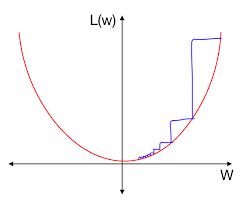
\includegraphics[width=40mm]{Images/GradientDescent.png}   
  \hspace{3mm}
  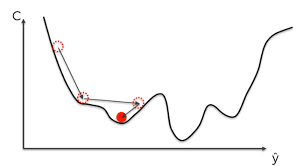
\includegraphics[width=50mm]{Images/LocalMinima.png}   
\end{center}

Gradient descent requires a good starting point and an energy
landscape with no local minima.
\end{frame}


%-------------------------------------------------------------------
\begin{frame} 
To avoid oscilations (running zig-zag down
through a narrow valley) often a momentum parameter is included:

\begin{displaymath}
  x^{n+1} \;=\; x^n - \nu \nabla f(x^n) - \epsilon \nabla f{x^{n-1}}
\end{displaymath}

\begin{center}
  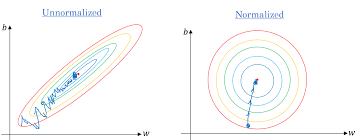
\includegraphics[width=90mm]{Images/Momentum.png}   
\end{center}

Momentum may accelerate convergence by smoothing out oscillations.

\end{frame}


%-------------------------------------------------------------------
% \begin{frame} 
%   \frametitle{Autograd}
% {\color{blue}{The pytorch autograd package}} is a system for automatic
% differentiation (gradient computation) for all operations on
% {\color{blue}{tensors}}. A tensor may be seen as a generalization of a
% matrix to 3D. This is the tool for optimizing NNs, but have wider
% application areas. \\[6mm] 
%
% To appreciate Autograd you first need to understand backpropagation.
% However, you may check out {\color{green}{pytorch}} and the use of
% tensors (e.g. Google GettingStarted with PyTorch).
% \end{frame}


%-------------------------------------------------------------------
\begin{frame} 
  \frametitle{Stochastic optimization}
The purpose of stochastic optimization is to avoid getting trapped in
local minima. Depending on the framework, it may show up in many
ways. \\[4mm]

In NN-learning we could (in theory) compute the error (which we will
back-propagate through the net) from all training data.  It would be
robust (i.e. identifying the right direction) but would be very
slow. \\[4mm]

As alternative, a single sample could form the basis for error
propagation. This would be fast, but extremely noisy and risky. \\[4mm]

In between, we may select a {\color{blue}{mini-batch}} including say
4-256 random samples (i.e. images). 
  \end{frame}



%-------------------------------------------------------------------
\begin{frame} 
  \frametitle{Mini-batches and batch size}

  The larger the bach-size the better (more stable/robust) gradient
  for error propagation,   but the more work per iteration. \\[4mm]

  It is not clear, given a net and a task, what batch size is optimal.
  What is clear is that smaller baches require more iterations for
  convergence. \\[4mm]

  If using small batch-sizes, a small larning rate, and use of
  momentum becomes essential. \\[4mm]

  Using large mini-batches may not be possible because of storage
  limitations in GPU's.
  
\end{frame}


%-------------------------------------------------------------------
\begin{frame} 
  \frametitle{SGD, ADAM etc}
SGD is a standard NN-optimization framework where the user specifies
the batch size, learning rate, momentum etc.  Then, given training
(and validation data) it optimizes the {\color{blue}{loss function}}
during a number of {\color{blue}{epochs}}, each including as many
iterations as necessary for covering the hole set of training
data. \\[3mm]

The user also specifies the maximum number of epochs and if the
training rate should be lowered after each sequence of $n$
epochs. \\[3mm] 

For an initial high learning rate, the movent in the energy landscape
is large, probably bypassing the global minimum. Lowering the learning
rate ensures that the locally deepest minimum is found. \\[3mm]

Usually the choice of optimizer does not change the result (the
minimum). Instead one optimizer may work/converge where another will
diverge.  

\end{frame}


%-------------------------------------------------------------------
\begin{frame}
\frametitle{Chosing and lowering the learning rate}
   
\begin{center}
  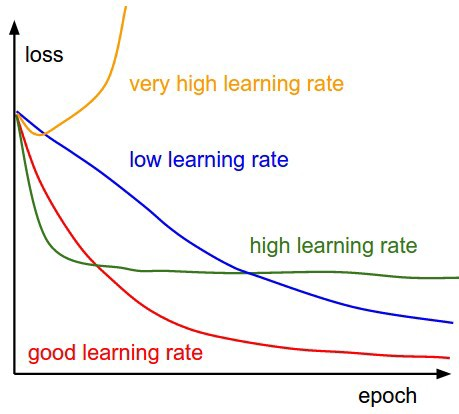
\includegraphics[width=50mm]{Images/Learningrate1.jpeg}
  \hspace{3mm}
  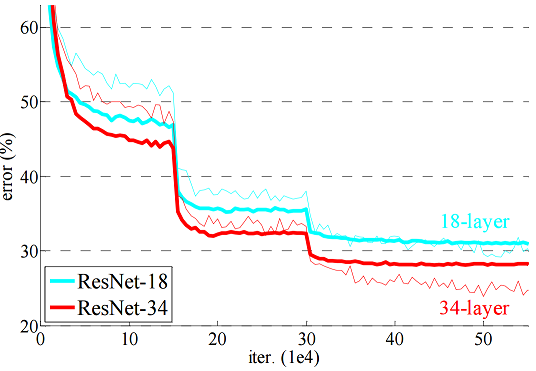
\includegraphics[width=50mm]{Images/learningrate2.png}  
\end{center}

\end{frame}


%-------------------------------------------------------------------
\begin{frame} 
  \frametitle{Class exercise (0.5 minute)}
  \vspace{15mm}
  
  \color{blue}{{\Large \bf
      Overfitting happens when a too complex/expressive model is
      fitted to a too simple dataset.  \\[8mm]

      Figure out a method to detect when overfitting happens.
    }}
    
  
\end{frame}


%-------------------------------------------------------------------
\begin{frame} 
  \frametitle{Training, validation and test data}
When training a CNN, {\color{red}{\bf never}} use all data.  Always keep
back a test set, locked away and never used before {\color{red}{all}}
development is over.  Often the test set includes say 10-15\% of the
data. \\[5mm]

To train the network it is of vital impotance to avoid overfitting. To
monitor that 10-15\%  is held back for validation.  For each training
epoch, the net is validated on this set. If the validation error is
much larger than the training error, overfitting takes place and the
training has failed. \\[5mm]

If the validation error tend to increase {\color{red}{early stopping}}
may be used to avoid further overfitting.

 \end{frame}



%-------------------------------------------------------------------
 \begin{frame}
   
\begin{center}
  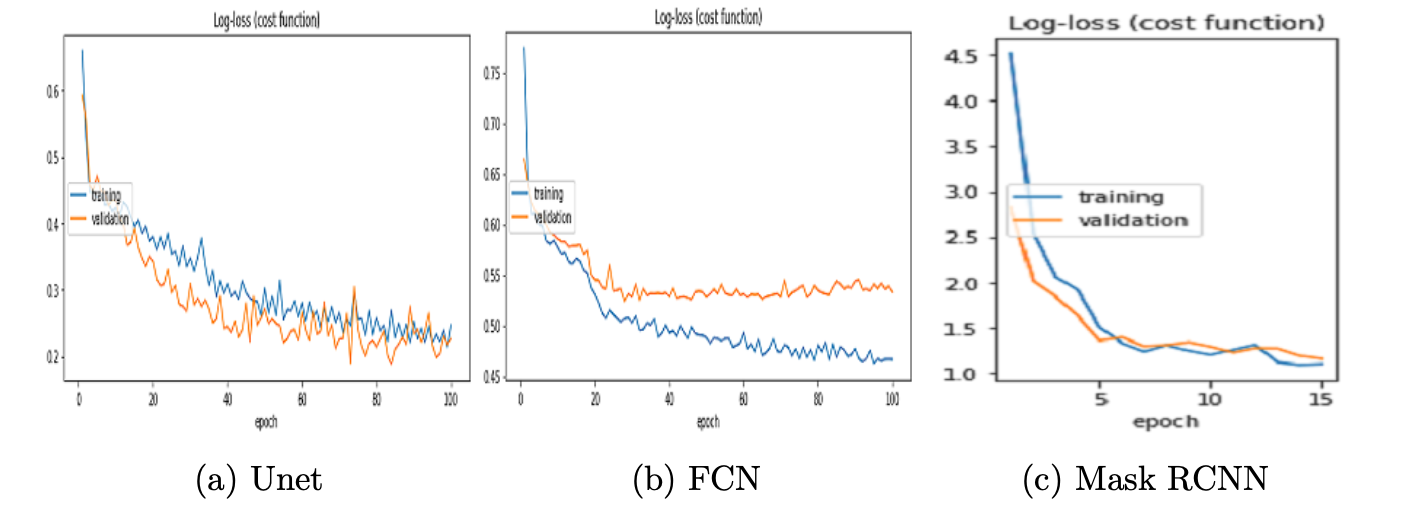
\includegraphics[width=110mm]{Images/validation.png}   
\end{center}
\bigskip

Overfitting takes place when the validation error flattens out while
the training error keeps decreasing.

 \end{frame}



%-------------------------------------------------------------------
% \begin{frame} 
%   \frametitle{Next}
%   \begin{itemize}
%   \item Loss functions,
%   \item Pretraining and transfer learning
%     % \item The backpropagation algorithm (if I can make it)\\[5mm]
%   \item (A corner of) the zoo of net architectures \\[5mm]
% %  \item Prepare first draft of a your table of contents for your report
%   \end{itemize}
% \bigskip
%
% Prepare by reading, in particular on backpropagation. Also,
% Please, each of you:  Prepare a question for me. On a topic or assignment.
%
% \end{frame}



%-------------------------------------------------------------------
\begin{frame} 
  \frametitle{What to optimize}
  \begin{itemize}
    \item The {\color{blue}{loss-function}} specifies what to be
      optimized \\[3mm]
    \item The loss function should be differentiable \\[3mm]
    \item Cross-Entropy is usually used for classification \\[3mm]
    \item L2-norm usually used for regression \\[3mm]
    \item The loss function may contain a number terms and may be
      designed to put weight on rare or difficult cases/classes. \\[6mm]
    \end{itemize}

    More on loss-functions in a another set of slides.
 \end{frame}


 

\end{document}


